\documentclass{beamer}
\usetheme{Berlin}

\begin{document}
\title{Grupo de trenzas y su aplicación en criptografía}   
\author{Fernando de la Hoz Moreno} 
\date{\today} 

\frame{\titlepage} 

\frame{\frametitle{Table of contents}\tableofcontents} 


\section{Grupo de trenzas}


\begin{frame}
\frametitle{Emil Artin} 

\begin{minipage}{.5\textwidth}

\begin{itemize}
\item Matemático austriaco (1898-1962).
\item Universidad de Gotinga y Universidad de Princeton.
\item Teoría de números, teoría algebraica de anillos asociativos y en los números hipercomplejos.
\item Acuñó los términos \textit{trenza} y \textit{grupo de trenzas} por primera vez en el año 1925.
\end{itemize}


\end{minipage}\hfill
\begin{minipage}{.5\textwidth}
\begin{figure}
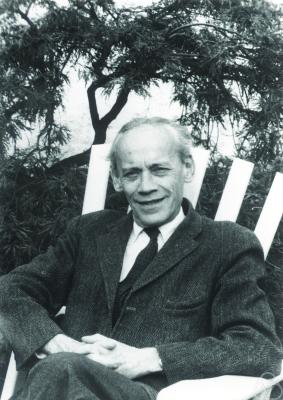
\includegraphics[height=0.9\textwidth]{imgs/EmilArtin}
\caption{Fotografía de Emil Artin \cite{}.}
\end{figure}
\end{minipage}

\end{frame}





\begin{frame}
\frametitle{Grupo de trenzas de Artin}

El \textit{grupo de trenzas de Artin} $B_n$ es el grupo generado por $n-1$ elementos $\sigma_1, \sigma_2,...,\sigma_{n-1}$ y las relaciones de trenza
$$\sigma_i\sigma_j = \sigma_j\sigma_i,$$
para todo $i,j\in\{1,2,...,n-1\}$ con $|i-j|\geq 2$ y

$$\sigma_i\sigma_{i+1}\sigma_i =\sigma_{i+1}\sigma_i\sigma_{i+1},$$
para todo $i\in\{1,2,...,n-2\}$.

\end{frame}



\begin{frame}
\frametitle{Trenza Geométrica}

Una trenza geométrica de $n$ hebras, con $n \geq 1$, es un subconjunto $\mathcal{B}\subset\mathbb{R}^2\times I$ formado por $n$ intervalos topológicos (subconjuntos de $\mathbb{R}^2\times I$ homeomorfos al intervalo $[0,1]$) disjuntos llamados hebras de tal manera que la proyección $\mathbb{R}^2\times I\rightarrow I$ establezca un homeomorfismo de cada hebra en $I$ y
$$\mathcal{B}\cap(\mathbb{R}^2\times \{0\})=\{(1,0,0),(2,0,0),...,(n,0,0)\},$$
$$\mathcal{B}\cap(\mathbb{R}^2\times \{1\})=\{(1,0,1),(2,0,1),...,(n,0,1)\}.$$
Cada hebra de $\mathcal{B}$ interseca con el plano $\mathbb{R}^2\times \{t\}$ con $t\in I$ en un único punto y conecta un punto $(i,0,0)$ con un punto $(s(i),0,1)$ donde $i,s(i)\in\{1,2,...,n\}$. La sucesión $(s(1),s(2),...,s(n))$ es una permutación del conjunto $\{1,2,...,n\}$ llamada permutación subyacente de $\mathcal{B}$.
\end{frame}



\begin{frame}
\frametitle{Trenza Geométrica}

\begin{figure}
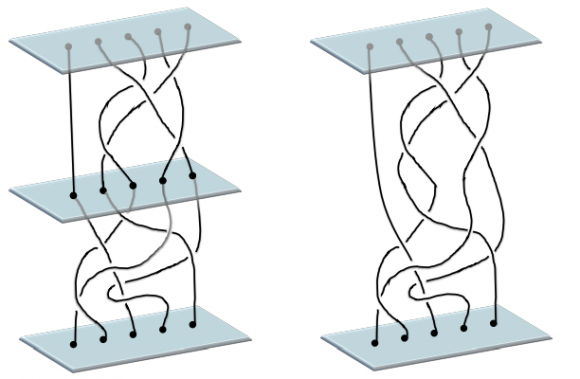
\includegraphics[height=0.5\textwidth]{imgs/trenza_geo}
\caption{Trenza Geométrica \cite{}.}
\end{figure}

\end{frame}






\section{Section} 
\frame{\frametitle{Title} 
Each frame should have a title.
}
\subsection{Subsection no.1.1  }
\frame{ 
Without title somethink is missing. 
}


\section{Section no. 2} 
\subsection{Lists I}
\frame{\frametitle{unnumbered lists}
\begin{itemize}
\item Introduction to  \LaTeX  
\item Course 2 
\item Termpapers and presentations with \LaTeX 
\item Beamer class
\end{itemize} 
}

\frame{\frametitle{lists with pause}
\begin{itemize}
\item Introduction to  \LaTeX \pause 
\item Course 2 \pause 
\item Termpapers and presentations with \LaTeX \pause 
\item Beamer class
\end{itemize} 
}

\subsection{Lists II}
\frame{\frametitle{numbered lists}
\begin{enumerate}
\item Introduction to  \LaTeX  
\item Course 2 
\item Termpapers and presentations with \LaTeX 
\item Beamer class
\end{enumerate}
}
\frame{\frametitle{numbered lists with pause}
\begin{enumerate}
\item Introduction to  \LaTeX \pause 
\item Course 2 \pause 
\item Termpapers and presentations with \LaTeX \pause 
\item Beamer class
\end{enumerate}
}

\section{Section no.3} 
\subsection{Tables}
\frame{\frametitle{Tables}
\begin{tabular}{|c|c|c|}
\hline
\textbf{Date} & \textbf{Instructor} & \textbf{Title} \\
\hline
WS 04/05 & Sascha Frank & First steps with  \LaTeX  \\
\hline
SS 05 & Sascha Frank & \LaTeX \ Course serial \\
\hline
\end{tabular}}


\frame{\frametitle{Tables with pause}
\begin{tabular}{c c c}
A & B & C \\ 
\pause 
1 & 2 & 3 \\  
\pause 
A & B & C \\ 
\end{tabular} }


\section{Section no. 4}
\subsection{blocs}
\frame{\frametitle{blocs}

\begin{block}{title of the bloc}
bloc text
\end{block}

\begin{exampleblock}{title of the bloc}
bloc text
\end{exampleblock}


\begin{alertblock}{title of the bloc}
bloc text
\end{alertblock}
}
\end{document}